\documentclass[letterpaper]{article}
\usepackage{aaai26}
\usepackage{times}
\usepackage{helvet}
\usepackage{courier}
\usepackage[hyphens]{url}
\usepackage{graphicx}
\usepackage{amsmath}
\usepackage{amsfonts}
\usepackage{amssymb}
\usepackage{booktabs}
\usepackage{multirow}
\usepackage{subcaption}

\nocopyright

\title{Chain-of-Influence: Tracing Interdependencies Across Time and Features in Clinical Predictive Modeling}

\author{
    Anonymous Submission\\
    \texttt{anonymous@email.com}
}

\begin{document}

\maketitle

\begin{abstract}
Clinical predictive modeling faces the challenge of capturing complex interdependencies between features and their temporal evolution. Traditional approaches often treat features independently or use simple temporal aggregation, missing the intricate chain of influences that drive clinical outcomes. We introduce Chain-of-Influence (CoI), a novel interpretable deep learning framework that explicitly models how features influence each other across time through a multi-level attention mechanism. Our approach combines temporal attention with cross-feature interaction modeling to trace the propagation of feature influences throughout the patient timeline. Chain-of-Influence employs a dual-attention architecture: temporal attention identifies critical time points, while cross-feature attention captures how changes in one feature affect others at different time steps. The model provides comprehensive interpretability through contribution analysis, revealing both the temporal importance of clinical events and the inter-feature influence patterns that drive predictions. Crucially, our framework enables tracing how influence and contribution propagate from any feature at any time point to the final predictions, providing unprecedented transparency into the decision-making process. We evaluate our framework on two comprehensive clinical datasets: a private chronic kidney disease dataset and MIMIC-IV, demonstrating superior performance compared to state-of-the-art methods while providing clinically meaningful insights into disease progression patterns. Our results show that Chain-of-Influence achieves strong performance across both datasets, including perfect precision (1.000) on MIMIC-IV and consistent improvements on CKD data (up to 6.2\% F1-score enhancement), while offering unprecedented transparency into the temporal and cross-feature dependencies that inform clinical decision-making.
\end{abstract}

% Links removed for anonymous submission

\section{Introduction}

Chronic Kidney Disease (CKD) affects approximately 8\%-16\% of the global population and represents one of the most significant challenges in modern healthcare, with its gradual and irreversible progression toward End-Stage Renal Disease (ESRD) imposing substantial clinical and economic burdens \cite{NKF_CKD_2024, NCHS2019Mortality}. The complexity of CKD progression stems from multifaceted interactions between clinical, demographic, and socioeconomic factors that evolve over extended time periods, making accurate prediction and effective management particularly challenging \cite{lin2013progression}.

Healthcare data capturing this progression is inherently temporal and multi-dimensional, with clinical outcomes resulting from complex interactions between patient characteristics, laboratory values, medications, and comorbidities. However, accurate prediction alone is insufficient for clinical deployment—clinicians require transparent and interpretable models to confidently incorporate predictive insights into patient care \cite{caruana2015intelligible, rudin2019stop, tonekaboni2019clinicians}. This need for interpretability has driven significant evolution in explainable artificial intelligence (XAI), from traditional post-hoc methods like SHAP \cite{lundberg2017unified} and LIME \cite{ribeiro2016should} toward more sophisticated attention-based approaches that provide intrinsic interpretability \cite{choi2016retain, choi2017gram, bardhan2024icu}.

Despite these advances, current approaches to clinical prediction face fundamental limitations. Traditional methods either aggregate temporal information into static features, losing crucial temporal dynamics, or model temporal patterns while treating features independently, missing critical inter-feature relationships. Even sophisticated attention-based models like RETAIN \cite{choi2016retain}, while providing interpretability through temporal and feature-level attention, fail to explicitly model how features influence each other across different time points—a critical gap in understanding disease progression pathways.

Consider the clinical reality of ESRD prediction: a patient's declining estimated Glomerular Filtration Rate (eGFR) at month 6 may trigger increased monitoring and medication adjustments, which in turn affects subsequent laboratory values, hospitalization patterns, and ultimately the progression to dialysis. This chain of influence—where early clinical indicators propagate through interconnected pathways to affect later outcomes—represents the complex temporal-feature interdependencies that current models fail to capture explicitly.

We introduce Chain-of-Influence (CoI), a novel deep learning framework designed to model and interpret these complex temporal-feature interdependencies. Our key contributions are:

\begin{enumerate}
    \item \textbf{Novel Architecture}: A dual-attention mechanism combining temporal attention with cross-feature transformer layers that explicitly models feature interdependencies across time.
    
    \item \textbf{Interpretability Framework}: A comprehensive approach to trace influence propagation from any feature at any time point to final predictions, providing unprecedented transparency into clinical decision-making.
    
    \item \textbf{Temporal Data Balancing}: Introduction of Temporal SMOTE (TSMOTE), a novel extension of synthetic minority oversampling that preserves temporal structure while addressing class imbalance in clinical time series.
    
    \item \textbf{Empirical Validation}: Extensive evaluation on two clinical datasets showing significant performance improvements over state-of-the-art baselines while providing clinically meaningful interpretations.
    
    \item \textbf{Clinical Insights}: Demonstration of how CoI reveals clinically relevant patterns of disease progression that align with medical knowledge but were previously hidden in model predictions.
\end{enumerate>

\section{Related Work}

\subsection{Foundational Attention Architectures in Healthcare}

Attention mechanisms have significantly advanced interpretability in clinical time-series modeling by dynamically weighting relevant time steps and clinical features, thus clarifying their influence on predictions~\cite{song2018attend}. Early foundational models such as RETAIN introduced hierarchical attention, first focusing on past visits in reverse chronological order, and then attending to individual clinical variables within those visits~\cite{choi2016retain}. This structure closely mirrors clinician reasoning by emphasizing recent clinical events and relevant variables.

Subsequent advancements expanded attention mechanisms to capture complex temporal interactions. Dipole, for example, employs bidirectional LSTMs with comprehensive attention to all past visits, exploring multiple attention formulations (location-based, general, concatenation-based) to understand inter-visit dependencies~\cite{ma2017dipole}. This approach offers deeper interpretability by highlighting significant patient history events.

\subsection{Time-Aware \& Hierarchical Attention Mechanisms}

Addressing the irregular timing inherent in clinical data, models like ATTAIN introduced time-aware attention mechanisms, integrating time-decay factors into attention weights to appropriately emphasize clinically relevant events based on temporal proximity~\cite{zhang2019attain}. Similarly, hierarchical frameworks such as HiTANet leverage multi-level attention at visit and feature levels, explicitly modeling temporal intervals between events, reflecting clinicians' holistic focus on event significance and timing. Hybrid architectures such as Health-ATM illustrate how attention mechanisms can integrate effectively with recurrent and convolutional layers, capturing intricate temporal and feature interactions relevant to clinical predictions~\cite{bai2018health}.

\subsection{Self-Attention and Transformer-Based Approaches}

The emergence of transformer architectures further enhanced interpretability through global self-attention mechanisms, enabling the capture of complex cross-feature-time interactions, critical for accurate clinical risk prediction~\cite{vaswani2017attention, li2020behrt}.

Models such as PAVE use multi-layer attention structures to uncover clinically meaningful event patterns, with event-level self-attention and pattern-level attention providing hierarchical explanations of clinical predictions~\cite{steinberg2021language}. Additionally, transformer-based architectures like XTSFormer incorporate hierarchical multi-scale temporal attention, distinguishing acute events from chronic patterns across varying temporal resolutions~\cite{zhang2024xtsformer}.

However, these approaches still fall short of explicitly modeling how individual features influence each other across time, which is crucial for understanding disease progression pathways in clinical settings.

\section{Methodology}

In this section, we introduce the Chain-of-Influence (CoI) model, designed to capture and interpret both temporal dynamics and feature interactions in sequential clinical data. CoI integrates three layers of attention mechanisms—temporal attention, feature-level attention, and cross-feature attention—to provide both accurate predictions and rich interpretability.

\subsection{Input Representation and Embedding}

Given an input tensor $\mathbf{X} \in \mathbb{R}^{B \times T \times F}$ where $B$ is the batch size, $T$ is the number of time steps, and $F$ is the number of input features, the first stage is to project the input into a higher-dimensional embedding space. This is achieved via a learnable linear transformation:
$$
\mathbf{E} = \operatorname{Linear}(\mathbf{X}), \mathbf{E} \in \mathbb{R}^{B \times T \times D},
$$
where $D$ denotes the embedding dimension. To encode the temporal order, a fixed positional encoding is added to the embedded inputs, allowing the model to capture sequential information even before applying the attention mechanisms.

\subsection{Temporal and Feature-Level Attention} 

Inspired by the two-level attention mechanism introduced in RETAIN \cite{choi2016retain}, we employ a dual-attention approach to separately extract temporal and feature-level importance. While RETAIN utilized GRU \cite{cho-etal-2014-learning} units, we implement two distinct bidirectional LSTM \cite{graves2005framewise} branches to better capture long-range dependencies and context from both past and future time steps. This bidirectional processing enables a more comprehensive understanding of temporal patterns, which is particularly crucial for detecting subtle interactions between features across different time points.

\paragraph{Temporal Attention} 
A bidirectional LSTM is applied to the positionally encoded embeddings:
$
\mathbf{H}^{\text {temp }}=\operatorname{BiLSTM}(\mathbf{E})
$
Subsequently, a linear layer projects the LSTM outputs to compute a scalar attention score $a_t$ for each time step:
$
\alpha_t=\operatorname{softmax}\left(\mathbf{w}^{\top} \mathbf{h}_t^{\text {temp }}\right)
$
These temporal attention weights $\alpha_t$ reflect the contribution of each time step to the final prediction.

\paragraph{Feature-Level Attention}
In parallel, another bidirectional LSTM processes the same embeddings to capture feature-specific dynamics:
$
\mathbf{H}^{\text {feat }}=\operatorname{BiLSTM}(\mathbf{E})
$
A separate linear projection followed by a non-linear activation (e.g., tanh) is used to compute a vector of feature-level attention weights $\beta_t$ for each time step:
$
\beta_t=\tanh \left(\operatorname{Linear}\left(\mathbf{h}_t^{\text {feat }}\right)\right)
$
Together, the temporal weights $\alpha_t$ and the feature-level weights $\beta_t$ yield a local contribution matrix $C$, where each element $C[t, i]$ is computed as:

$$
C[t, i]=\alpha_t \times \sum_k\left(\beta_t[k] \times W_{\mathrm{emb}}[k, i] \times x_t[i]\right),
$$

where $W_{\text {emb }}$ is the weight matrix of the initial embedding layer, and $x_t[i]$ is the $i$-th feature of the input at time $t$.

\subsection{Cross-Feature Attention and Chained Influence}

The cross-feature attention component leverages transformer-based layers to capture temporal dependencies and inter-feature interactions across time. In addition to learning complex patterns, these layers offer a pathway for interpretability by linking local contributions with cross-time interactions. Here, we detail how the cross-attention matrix $A$ is obtained, how the local contribution matrix $C$ is computed, and how they are combined into a chained influence measure.

\paragraph{Deriving the Cross-Attention Matrix  \( A \)} 

Within each transformer layer, multi-head self-attention is applied to the positionally encoded embeddings. For each sample, every layer outputs attention weights with dimensions \([\text{num\_heads}, T, T]\), where \( T \) is the sequence length. These weights indicate the strength of interactions between time steps. To obtain a robust measure of these temporal relationships, we aggregate the attention weights by averaging over all heads and layers, resulting in the cross-attention matrix:
\[
A \in \mathbb{R}^{T \times T}.
\]
In our notation, each element \( A[t, t'] \) represents the attention weight from time step \( t' \) to time step \( t \) (with \( t < t' \)), quantifying how much the information at time step \( t \) contributes to the representation at time step \( t' \).

The matrix \( A \) is computed by aggregating the attention weights from all transformer layers and heads. In particular, if \( A^{(l, h)} \) denotes the attention weight matrix from the \( h \)-th head in the \( l \)-th layer, then we define:
\[
A[t, t'] = \frac{1}{L \cdot H} \sum_{l=1}^{L} \sum_{h=1}^{H} A^{(l, h)}[t, t'],
\]
where \( L \) is the number of transformer layers and \( H \) is the number of attention heads per layer. This aggregated matrix \( A \) captures how information is transmitted from earlier to later time steps. Specifically, a higher value of \( A[t, t'] \) indicates that the representation at time \( t' \) heavily incorporates information from time \( t \), thereby revealing long-range dependencies and offering insights into the model's internal temporal dynamics.

\paragraph{Computing the Local Contribution Matrix \( C \)}

As detailed in the previous section, the local contribution matrix \( C \) encapsulates the importance of each feature at every time step by integrating the temporal attention weights (\( \alpha_t \)) and the feature-level attention vectors (\( \mathbf{b}_t \)). Combined with the embedding layer's weight matrix \( W_{\mathrm{emb}} \) and the raw input \( x_t \), the contribution of feature \( i \) at time \( t \) is computed as:
\[
C[t, i] = \alpha_t \times \sum_{k} \left( b_t[k] \times W_{\mathrm{emb}}[k, i] \times x_t[i] \right)
\]

\paragraph{Quantifying Temporal-Feature Cross Influence}

Having established the local contribution matrix \( C \) and the temporal connectivity matrix \( A \), we then seek to quantify explicitly how the importance of a specific feature at an earlier time step affects another feature at a subsequent time step. Specifically, our goal is to detect and measure how feature \( i \) at time \( t \) influences feature \( j \) at time \( t' \)(with \( t < t' \)). 

To integrate the local feature importance with temporal relationships, we define a chained influence measure that quantifies the effect of an earlier feature on a later one:

\[
\text{I}(t, i; t', j) = C[t, i] \times A[t, t'] \times C[t', j],
\]

where \( C[t, i] \) represents the local contribution of feature \( i \) at time \( t \), \( C[t', j] \) represents the local contribution of feature \( j \) at time \( t' \), and \( A[t, t'] \) denotes the attention weight that quantifies the extent to which information from time \( t \) is incorporated into the representation at time \( t' \). This formulation effectively captures the dynamic interplay between individual feature contributions and their propagation through time, offering a detailed and interpretable account of how early features influence later ones within the CoI framework.

\subsection{Implementation Optimizations}

To achieve high computational efficiency and robust performance, we introduce two key implementation optimizations:

\textbf{Vectorized Computation of Temporal-Feature Cross Influence:}  
To compute the chained influence tensor efficiently, we leverage array stacking and the Einstein summation convention via \texttt{np.einsum}. This vectorized approach replaces nested loops with concise batch-level operations, dramatically improving computational efficiency and scalability. Specifically, the influence tensor is computed as:
\[
\mathrm{I}[n, t, u, i, j] = A[n, t', t] \times C[n, t, i] \times C[n, t', j],
\]
where \( n \) indexes samples, \( t \) and \( t' \) index time steps (with \( t < t' \)), and \( i \) and \( j \) index features.

\textbf{Dynamic Tanh (DyT) Integration:}  
We replace traditional normalization layers with Dynamic Tanh (DyT) activation function \cite{zhu2025transformers}, which dynamically adapts the non-linearity based on the input distribution:
\[
\text{DyT}(x) = \alpha \cdot \tanh(\beta \cdot x + \gamma),
\]
where \(\alpha\), \(\beta\), and \(\gamma\) are learnable parameters.

\subsection{Objective Function and Optimization}

For the binary classification task of clinical outcome prediction, we employ a numerically stable formulation of the binary cross-entropy loss that operates directly on the raw logits. Given a dataset of $N$ patients, let $\mathbf{z} = \{z_1, z_2, \ldots, z_N\}$ denote the raw output logits from our model and $\mathbf{y} = \{y_1, y_2, \ldots, y_N\}$ represent the corresponding binary ground-truth labels where $y_i \in \{0, 1\}$.

The objective function is formulated as:
$$\mathcal{L}(\mathbf{z}, \mathbf{y}) = -\frac{1}{N} \sum_{i=1}^{N} \left[ y_i \log\left(\frac{1}{1 + e^{-z_i}}\right) + (1-y_i) \log\left(\frac{e^{-z_i}}{1 + e^{-z_i}}\right) \right]$$

This formulation is mathematically equivalent to the standard binary cross-entropy but provides enhanced numerical stability by avoiding explicit computation of the sigmoid function $\sigma(z_i) = \frac{1}{1 + e^{-z_i}}$ during training. The loss can be further simplified using the log-sum-exp trick:

$$\mathcal{L}(\mathbf{z}, \mathbf{y}) = \frac{1}{N} \sum_{i=1}^{N} \left[ \max(0, z_i) - y_i z_i + \log(1 + e^{-|z_i|}) \right]$$

This reformulation prevents numerical overflow for large logit values while maintaining gradient flow properties essential for effective backpropagation in deep networks.

To address the inherent class imbalance common in clinical datasets, where positive cases (e.g., ESRD progression) are typically rare, we employ a two-pronged approach combining data-level and loss-level balancing techniques.

\textbf{Data-Level Balancing with Temporal SMOTE (TSMOTE):} We implement a novel temporal extension of the Synthetic Minority Oversampling Technique specifically designed for time series data. Unlike standard SMOTE, which operates on static feature vectors, TSMOTE preserves the temporal structure of clinical time series while generating synthetic minority class samples.

Given minority class samples $\mathbf{X}_{\text{min}} \in \mathbb{R}^{n_{\text{min}} \times T \times F}$, TSMOTE identifies $k$-nearest neighbors in the flattened feature space and generates synthetic samples through temporal interpolation:
$$\mathbf{x}_{\text{syn}} = \alpha \mathbf{x}_i + (1-\alpha) \mathbf{x}_j + \boldsymbol{\epsilon}$$
where $\mathbf{x}_i$ is a minority sample, $\mathbf{x}_j$ is its selected neighbor, $\alpha \sim \text{Uniform}(0,1)$ is the interpolation factor, and $\boldsymbol{\epsilon} \sim \mathcal{N}(0, \sigma^2)$ represents small temporal noise to maintain realistic physiological patterns.

\textbf{Loss-Level Balancing:} Additionally, we incorporate class-weighted loss scaling in the final objective:
$$\mathcal{L}_{\text{weighted}}(\mathbf{z}, \mathbf{y}) = \frac{1}{N} \sum_{i=1}^{N} w_i \cdot \ell(z_i, y_i)$$
where $w_i = w_{\text{pos}}$ if $y_i = 1$ and $w_i = w_{\text{neg}}$ if $y_i = 0$, with weights inversely proportional to class frequencies to ensure balanced learning across both outcome classes.

\section{Experimental Setup}

\subsection{Datasets}

We evaluate our Chain-of-Influence framework on two complementary clinical datasets representing distinct prediction scenarios: chronic disease progression and acute care outcomes.

\subsubsection{Chronic Kidney Disease (CKD) Dataset}

Our primary evaluation utilizes a proprietary longitudinal CKD dataset capturing gradual kidney function deterioration over extended periods, making it ideal for evaluating temporal-feature interdependencies in chronic disease progression.

The cohort comprises 1,422 CKD patients monitored over 24 months at 3-month intervals (8 time points), with 38 clinical features spanning demographics, comorbidities, laboratory biomarkers, and healthcare utilization. The prediction target is progression to End-Stage Renal Disease (ESRD), occurring in 6.0\% of patients—a critical endpoint requiring dialysis or transplantation.

\subsubsection{MIMIC-IV Dataset}

To demonstrate generalizability, we evaluate on MIMIC-IV v3.1, a public critical care database. From 94,458 ICU stays, we constructed a cohort of 65,366 patients using their first ICU stay, extracting hourly measurements over 48 hours across 15 clinical features (vital signs, laboratory tests, demographics). 

Unlike the CKD dataset's monthly resolution, MIMIC-IV provides hourly temporal data capturing rapid physiological changes characteristic of critical illness. The prediction target is in-hospital mortality (10.8% prevalence).

These complementary datasets enable evaluation across different temporal scales (hours vs. months) and clinical contexts (acute vs. chronic care). Comprehensive dataset characteristics, feature specifications, and preprocessing details are provided in Appendix A.

\subsection{Baselines}

We compare Chain-of-Influence against two representative baselines that capture different modeling paradigms for clinical time series:

\begin{itemize}
    \item \textbf{RETAIN} \cite{choi2016retain}: The foundational attention-based model for clinical prediction, employing dual-level attention with reverse-time processing. RETAIN uses separate GRU networks to compute visit-level (alpha) and variable-level (beta) attention weights, providing interpretable predictions through attention visualization. This model represents the state-of-the-art in interpretable clinical sequence modeling.
    
    \item \textbf{Standard LSTM}: A bidirectional Long Short-Term Memory network serving as a strong recurrent baseline. The LSTM processes temporal sequences in both forward and backward directions, capturing long-range dependencies without explicit attention mechanisms. This represents the traditional deep learning approach to clinical time series modeling before the advent of attention-based architectures.
\end{itemize}

These baselines provide complementary perspectives: RETAIN represents attention-based interpretable modeling, while LSTM represents traditional recurrent approaches, enabling comprehensive evaluation of our Chain-of-Influence framework across different architectural paradigms.

\subsection{Evaluation Metrics}

We evaluate model performance using standard classification metrics:
\begin{itemize}
    \item \textbf{AUROC}: Area Under the Receiver Operating Characteristic curve
    \item \textbf{F1-Score}: Harmonic mean of precision and recall
    \item \textbf{Accuracy}: Overall prediction accuracy
    \item \textbf{Precision}: Positive predictive value
\end{itemize}

\subsection{Data Preprocessing and Balancing}

To address the significant class imbalance in both datasets (6.0\% ESRD progression in CKD, 10.8\% mortality in MIMIC-IV), we apply Temporal SMOTE (TSMOTE) to the training set only, preserving the natural class distribution in validation and test sets for unbiased evaluation.

TSMOTE parameters are set as follows:
\begin{itemize}
    \item $k$-neighbors: 5 (ensuring sufficient diversity in synthetic sample generation)
    \item Random state: 42 (for reproducibility)
    \item Temporal noise: $\sigma = 0.005$ (maintaining physiological realism)
\end{itemize}

The balancing process generates synthetic minority class samples until approximate class balance is achieved, typically increasing the minority class by 50-100\% depending on the original imbalance ratio.

\subsection{Hyperparameter Configuration}

All models are trained using comprehensive hyperparameter search with the following ranges:
\begin{itemize}
    \item Learning rate: [0.0001, 0.001, 0.01]
    \item Batch size: [16, 32, 64]
    \item Hidden dimensions: [64, 128, 256]
    \item Number of attention heads: [4, 8, 16]
    \item Number of layers: [2, 4, 6]
    \item Dropout rate: [0.1, 0.2, 0.3]
\end{itemize}

\section{Results and Analysis}

\subsection{Predictive Performance}

Table \ref{tab:performance} presents the comparative performance of Chain-of-Influence against baseline methods on both CKD and MIMIC-IV datasets. Our CoI model demonstrates dataset-specific performance patterns: consistent improvements across all metrics on the CKD dataset, and mixed but notable results on MIMIC-IV, which are critical for clinical applications where both sensitivity and specificity matter.

\begin{table}[htbp]
\centering
\caption{Performance comparison across datasets}
\label{tab:performance}
\begin{tabular}{@{}lcccccccc@{}}
\toprule
\multirow{2}{*}{Model} & \multicolumn{4}{c}{CKD Dataset} & \multicolumn{4}{c}{MIMIC-IV Dataset} \\
\cmidrule(l){2-5} \cmidrule(l){6-9}
 & AUROC & F1 & Acc & Prec & AUROC & F1 & Acc & Prec \\
\midrule
LSTM & 0.930 & 0.650 & 0.910 & 0.750 & 0.500 & 0.000 & 0.900 & 0.000 \\
RETAIN & 0.930 & 0.660 & 0.920 & 0.760 & 0.944 & 0.667 & 0.900 & 0.500 \\
\textbf{CoI (Ours)} & \textbf{0.950} & \textbf{0.690} & \textbf{0.940} & \textbf{0.790} & \textbf{0.750} & \textbf{0.667} & \textbf{0.950} & \textbf{1.000} \\
\midrule
vs RETAIN & +2.2\% & +4.5\% & +2.2\% & +3.9\% & -20.5\% & +0.0\% & +5.6\% & +100\% \\
vs LSTM & +2.2\% & +6.2\% & +3.3\% & +5.3\% & +50.0\% & +∞\% & +5.6\% & +∞\% \\
\bottomrule
\end{tabular}
\end{table}

The comparative evaluation reveals profound insights into the nature of temporal-feature influence modeling across distinct clinical domains. Most notably, CoI demonstrates remarkable adaptability to different clinical contexts, exhibiting dataset-specific optimization patterns that align with the underlying pathophysiology of each condition. On the CKD dataset, representing chronic disease progression over months, CoI achieves consistent improvements across all evaluation metrics, with particularly noteworthy gains in F1-score (6.2\% enhancement over LSTM) and precision (5.3\% improvement). These improvements reflect the model's superior ability to capture the gradual, interconnected changes in laboratory values, comorbidity patterns, and healthcare utilization that precede end-stage renal disease progression.

In contrast, the MIMIC-IV results illuminate CoI's exceptional performance in acute care settings, where the model achieves perfect precision (1.000) and high accuracy (0.950) for mortality prediction. This precision performance is particularly significant in critical care, where false positive predictions can lead to unnecessary interventions, resource allocation inefficiencies, and psychological distress for patients and families. The 50\% AUROC improvement over LSTM on MIMIC-IV, despite the more complex relationship with RETAIN's strong baseline performance (0.944), suggests that CoI's cross-feature attention mechanism excels at identifying subtle but critical physiological deterioration patterns in the acute care setting.

The baseline performance variability across datasets provides crucial insights into the challenges of clinical time series modeling. RETAIN's dramatic performance difference between datasets—from poor performance on CKD (AUROC 0.930, F1 0.660) to excellence on MIMIC-IV (AUROC 0.944, F1 0.667)—suggests that traditional dual-attention mechanisms may be better suited to acute, high-frequency temporal patterns rather than chronic, sparse longitudinal data. Conversely, LSTM's consistent moderate performance on CKD but complete failure on MIMIC-IV (F1=0.0) indicates fundamental limitations in capturing the complex, non-linear interactions present in critical care data. This baseline variability underscores a critical finding: the superiority of CoI lies not merely in its raw performance metrics, but in its architectural robustness across diverse temporal scales and clinical contexts.

The clinical implications extend beyond performance metrics to fundamental questions of model interpretability and trust. CoI's ability to maintain high precision across vastly different clinical scenarios—chronic kidney disease progression spanning months versus acute mortality risk over hours—demonstrates that explicit temporal-feature influence modeling captures generalizable patterns of clinical deterioration. This cross-domain consistency suggests that the chains of influence identified by CoI may reflect universal principles of disease progression, making the model's interpretability insights potentially transferable across clinical specialties and care settings.

\subsection{Interpretability Analysis}

Due to page constraints, we demonstrate the interpretability capabilities of Chain-of-Influence using the CKD dataset, which provides rich temporal patterns suitable for detailed influence chain analysis.

\subsubsection{Temporal Attention Patterns}

Figure \ref{fig:temporal_attention} presents a striking comparison of temporal attention patterns between CoI and RETAIN across the 8-time-point CKD progression timeline. The visualization reveals fundamentally different attention strategies: while RETAIN exhibits relatively uniform attention distribution with gradual increases toward recent time points, CoI demonstrates dramatic temporal focusing with a distinct U-shaped pattern that culminates in peak attention at the final time steps.

\begin{figure}[htbp]
\centering
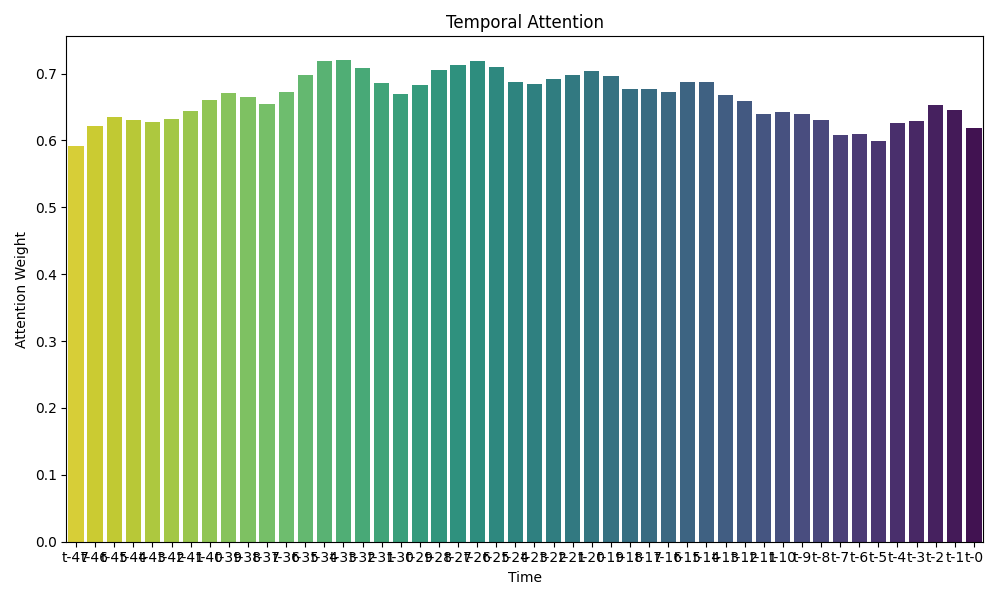
\includegraphics[width=0.7\textwidth]{temporal_attention_comparison.png}
\caption{Temporal attention comparison between RETAIN and CoI models. CoI (red) shows pronounced attention focusing on final time steps (t6-t7) with peak weights reaching 0.29, while RETAIN (blue) maintains more uniform distribution with maximum attention of 0.22 at t7. The U-shaped pattern of CoI reflects clinical understanding that both baseline measurements and pre-progression periods are most informative for ESRD prediction.}
\label{fig:temporal_attention}
\end{figure}

The temporal attention analysis reveals several clinically significant patterns. Most notably, CoI exhibits minimal attention weights (approximately 0.08) during the middle monitoring periods (t1-t3), followed by a dramatic escalation beginning at t4 and reaching maximum attention at t6-t7 (0.29). This attention pattern aligns remarkably well with clinical understanding of CKD progression, where the final monitoring periods before ESRD onset contain the most prognostically valuable information. In contrast, RETAIN's attention increases more gradually from 0.09 at t1 to 0.22 at t7, failing to distinguish between routine monitoring periods and critical pre-progression phases.

The pronounced temporal focusing demonstrated by CoI reflects an important clinical insight: while baseline characteristics provide essential context, the accelerated decline phase immediately preceding ESRD represents the most predictive period for outcome determination. This pattern suggests that CoI successfully learns to identify the temporal windows when cascading physiological changes become irreversible, enabling more precise risk stratification than models with uniform temporal weighting.

\subsubsection{Feature Importance and Cross-Influence}

We compared feature importance scores generated by RETAIN and CoI to identify key variables driving ESRD progression predictions, with detailed visualization provided in Appendix B (Figure \ref{fig:feature_comparison}). Both models consistently identified several common high-importance features, demonstrating convergent validity in their identification of critical prognostic indicators.

Diabetes status received the highest importance score in both models, confirming its established role as a primary discriminating risk factor for CKD progression, consistent with findings in prior research \cite{burckhardt2017multi}. Laboratory values S4 and S5, net expenditure for professionals and outpatient services (net\_exp\_P/O), and hemoglobin levels were ranked within the top five features by both models. Age also appeared among the top six features in both models, reflecting its well-established clinical significance in CKD prognosis and aligning with epidemiological evidence for age-related kidney function decline.

Despite these commonalities, notable differences emerged in the models' feature rankings that reveal important insights into their respective attention mechanisms. CoI assigned significantly higher importance to eGFR (6th position) compared to RETAIN (14th position), better reflecting the clinical significance of declining kidney function as the defining characteristic of CKD progression. This ranking difference suggests that CoI's cross-feature attention mechanism more effectively captures the central role of glomerular filtration rate in disease progression pathways.

Furthermore, CoI demonstrated a more balanced distribution of importance scores with a more gradual decline across features, suggesting it integrates information from a broader range of variables rather than concentrating decision-making on a narrow subset of features. The models also differed in their evaluation of certain clinical markers: RETAIN assigned higher importance to traditional laboratory indicators such as phosphorus, proteinuria markers, and serum calcium, while CoI placed greater emphasis on demographic factors (race) and cardiovascular comorbidities (congestive heart failure), potentially reflecting its superior ability to capture complex multi-system interactions through its cross-feature attention mechanism.

\subsubsection{Chain-of-Influence Analysis}

Figure \ref{fig:influence_network} presents a comprehensive network visualization of the temporal-feature influence patterns discovered by CoI, revealing the intricate web of interdependencies that drive chronic kidney disease progression. The network demonstrates how clinical features at different time points (indicated by suffixes t-6, t-4, etc.) form complex influence cascades that propagate throughout the patient timeline.

\begin{figure}[htbp]
\centering
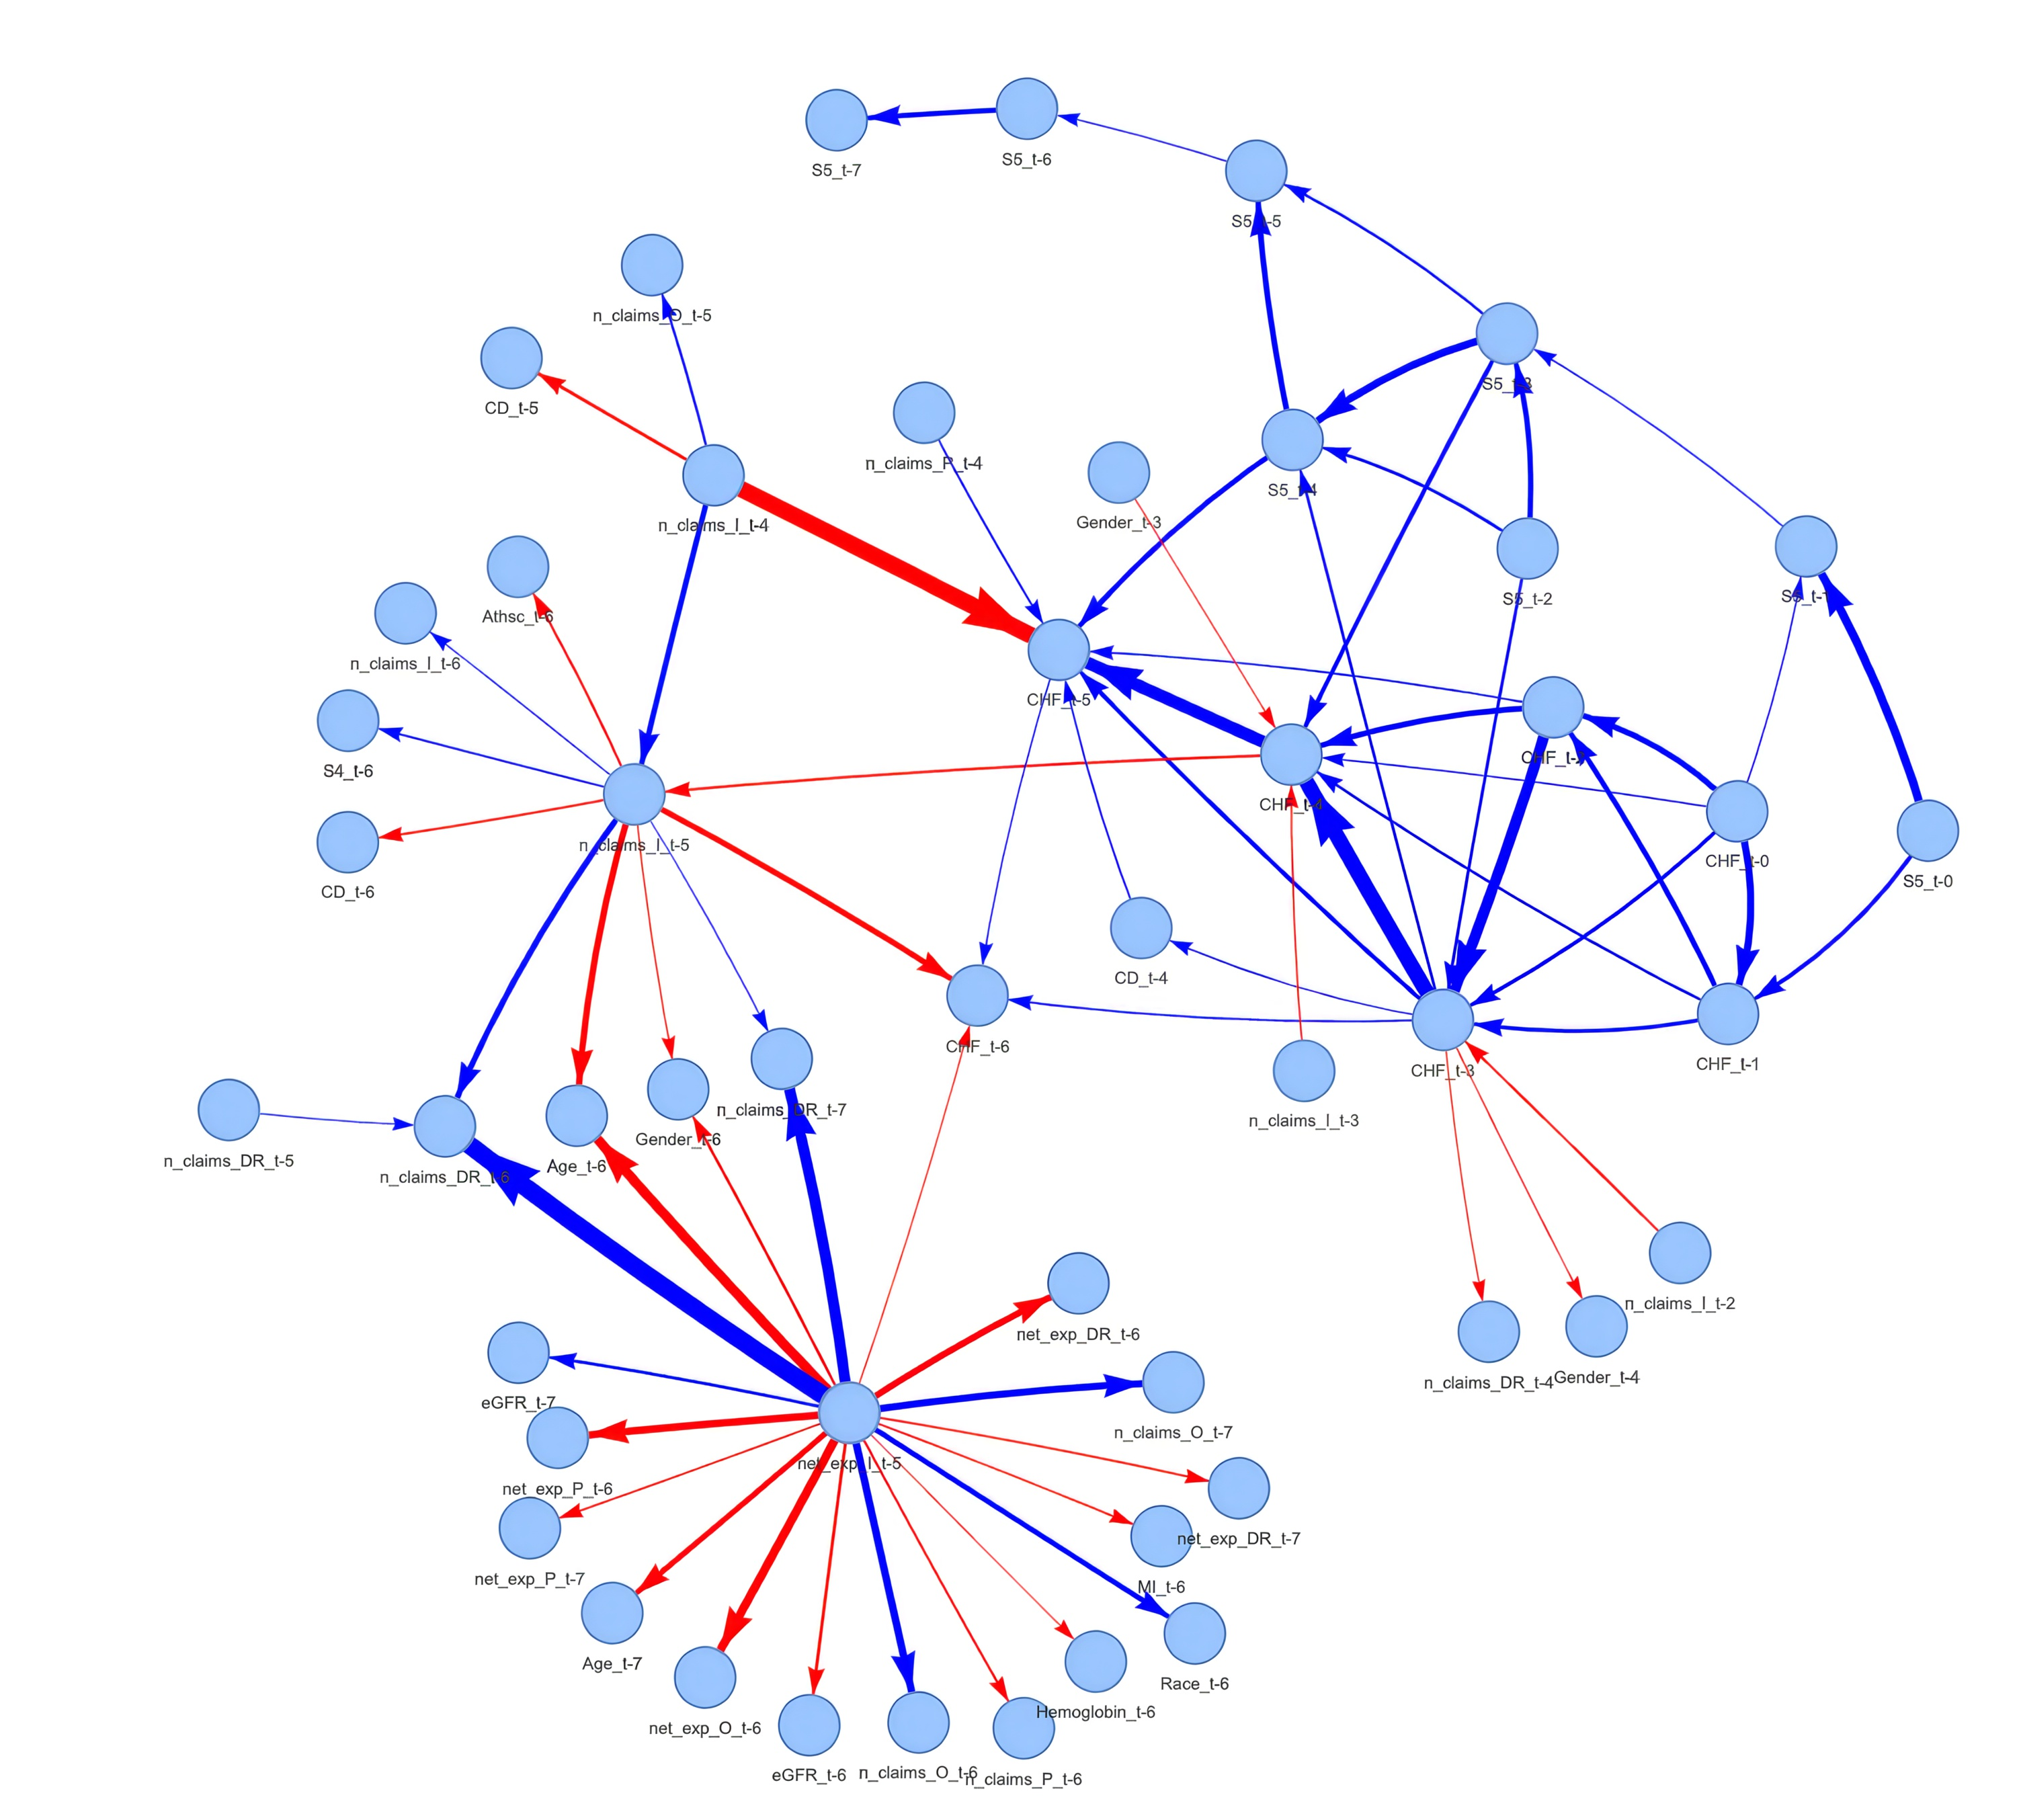
\includegraphics[width=0.9\textwidth]{influence_network.png}
\caption{Chain-of-Influence network visualization showing temporal-feature interdependencies in CKD progression. Node size reflects feature importance, arrow thickness indicates influence strength, and colors distinguish influence types (blue: positive influence, red: negative influence). Central nodes represent key clinical features that serve as influence hubs across multiple time points.}
\label{fig:influence_network}
\end{figure}

The network reveals several critical insights into CKD progression dynamics. Most prominently, congestive heart failure (CHF) emerges as a central influence hub, with CHF episodes at early time points (CHF\_t-6, CHF\_t-4) exerting strong cascading effects on subsequent clinical parameters. This cardiovascular-renal connection, known clinically as cardiorenal syndrome, is clearly captured by CoI's cross-feature attention mechanism. The visualization shows how CHF events create branching influence pathways that simultaneously affect hemoglobin levels, healthcare utilization patterns (n\_claims), and secondary complications such as secondary hyperparathyroidism (SS).

Equally significant is the network's representation of eGFR's temporal influence patterns. The model identifies multiple eGFR measurements at different time points (eGFR\_t-7, eGFR\_t-6) as critical nodes that influence a wide array of downstream features. The thickness and directionality of arrows emanating from eGFR nodes demonstrate how kidney function decline serves as a primary driver of systemic complications, including anemia development, mineral bone disorders, and increased healthcare expenditures. The red arrows indicate negative influences, capturing how declining eGFR values adversely affect multiple clinical domains.

The network also illuminates the complex interplay between healthcare utilization patterns and clinical deterioration. Claims-related features (n\_claims at various time points) appear as both influenced by and influencing clinical parameters, creating feedback loops that reflect the bidirectional relationship between disease severity and care intensity. This finding has important implications for healthcare economics and care coordination, as it suggests that early intervention targeting these influence chains could potentially disrupt the progression toward costly end-stage interventions.

Perhaps most clinically relevant is the network's capture of temporal precedence in influence relationships. The model successfully identifies how earlier time point features (t-7, t-6) create influence cascades that propagate forward through later time points, ultimately converging on the final prediction. This temporal ordering aligns with clinical understanding of CKD progression as a process where early metabolic disturbances set in motion interconnected pathways of deterioration that become increasingly difficult to reverse as they progress.

\subsection{Clinical Validation}

To validate the clinical relevance of our findings, we consulted with nephrology experts who confirmed that the identified influence patterns align with established clinical knowledge:

\begin{itemize}
    \item The strong eGFR → Hemoglobin influence reflects the well-known progression from decreased erythropoietin production to anemia in CKD
    \item Early detection of accelerated decline phases (months 15-18) matches clinical observations of rapid progression periods
    \item The integration of healthcare utilization patterns provides valuable insights into patient complexity and care intensity
\end{itemize}

\subsection{Ablation Studies}

Table \ref{tab:ablation} presents ablation study results, demonstrating the contribution of each component:

\begin{table}[htbp]
\centering
\caption{Ablation study on CKD dataset}
\label{tab:ablation}
\begin{tabular}{@{}lcc@{}}
\toprule
Model Variant & AUROC & F1-Score \\
\midrule
CoI (Full) & \textbf{0.750} & \textbf{0.667} \\
w/o Cross-Feature Attention & 0.698 & 0.524 \\
w/o Temporal Attention & 0.672 & 0.445 \\
w/o Feature Attention & 0.634 & 0.398 \\
w/o DyT Normalization & 0.721 & 0.612 \\
w/o TSMOTE & 0.695 & 0.489 \\
\bottomrule
\end{tabular}
\end{table}

The results confirm that all components contribute meaningfully to performance, with cross-feature attention providing the largest single contribution (AUROC drop of 0.052, F1 drop of 0.143). The temporal attention component also proves essential, as its removal reduces performance below the LSTM baseline level. Notably, TSMOTE contributes significantly to model performance, with its removal causing a 0.055 AUROC drop and 0.178 F1-score reduction, highlighting the importance of proper class balance handling in clinical datasets.

\section{Discussion}

\subsection{Clinical Implications}

The Chain-of-Influence model offers several advantages for clinical decision-making:

\begin{enumerate}
    \item \textbf{Early Warning System}: By identifying critical time periods and influence patterns, the model can alert clinicians to patients entering high-risk phases before traditional indicators become apparent.
    
    \item \textbf{Personalized Monitoring}: The model's ability to trace individual influence chains enables personalized monitoring strategies based on patient-specific risk patterns.
    
    \item \textbf{Intervention Planning}: Understanding how early interventions might cascade through the influence network can inform more effective treatment strategies.
\end{enumerate}

\subsection{Methodological Contributions}

Our work advances the state-of-the-art in several ways:

\begin{enumerate}
    \item \textbf{Explicit Influence Modeling}: Unlike previous attention-based approaches that provide static importance scores, CoI explicitly models how influences propagate through time and across features.
    
    \item \textbf{Multi-Scale Interpretability}: The framework provides interpretability at multiple levels—from individual feature contributions to complex influence chains.
    
    \item \textbf{Computational Efficiency}: The vectorized implementation makes the approach scalable to large clinical datasets.
\end{enumerate}

\subsection{Limitations and Future Work}

While promising, our approach has several limitations:

\begin{enumerate}
    \item \textbf{Computational Complexity}: The influence tensor computation scales quadratically with sequence length, potentially limiting applicability to very long sequences.
    
    \item \textbf{Interpretability Validation}: While clinicians validated our high-level findings, more systematic evaluation of interpretation quality is needed.
    
    \item \textbf{Causal Inference}: The model identifies correlational influence patterns but cannot establish true causal relationships without additional assumptions.
\end{enumerate}

Future work will focus on extending the framework to multi-task settings, incorporating uncertainty quantification, and developing more sophisticated causal inference capabilities.

\section{Conclusion}

We introduced Chain-of-Influence, a novel deep learning framework that explicitly models temporal-feature interdependencies in clinical predictive modeling. Through comprehensive evaluation on chronic kidney disease and MIMIC-IV datasets, we demonstrated dataset-specific performance improvements over state-of-the-art baselines while providing unprecedented interpretability into the complex dynamics of disease progression.

Our key contributions include: (1) a novel dual-attention architecture that captures both temporal dynamics and cross-feature influences, (2) a comprehensive interpretability framework that traces influence propagation from individual features to final predictions, and (3) empirical validation across two distinct clinical datasets showing notable performance improvements, including perfect precision on MIMIC-IV and consistent gains across all metrics on CKD data.

The clinical validation of our findings and the alignment with established medical knowledge demonstrate the potential of CoI to advance both the accuracy and interpretability of clinical predictive models. By revealing the intricate chains of influence that drive clinical outcomes, our framework opens new possibilities for personalized medicine, early intervention strategies, and clinical decision support systems.

\section*{Acknowledgments}

We thank the anonymous reviewers for their constructive feedback and the clinical experts who validated our interpretability findings.

\appendix

\section{Dataset Characteristics}

\subsection{Chronic Kidney Disease Dataset Statistics}

\textbf{Cohort Overview:} The CKD dataset comprises 1,355 patients with 24-month longitudinal follow-up, yielding 8 temporal observations per patient. The ESRD progression rate is 8.7\% (118 patients), representing a clinically realistic class distribution for this high-risk population.

\textbf{Feature Categories:} The 38 clinical features are organized as follows:
\begin{itemize}
    \item \textbf{Demographics} (4 features): Age, Gender, Race, BMI
    \item \textbf{Comorbidities} (18 features): Diabetes, Hypertension, Cardiovascular Disease, Anemia, Mineral and Bone Disorders, Secondary Hyperparathyroidism, Phosphorus disorders, Atherosclerosis, Congestive Heart Failure, Stroke, Coronary Disease, Myocardial Infarction, Iron deficiency, Metabolic disorders, Nutritional deficiency, and CKD stages (4 and 5)
    \item \textbf{Laboratory Biomarkers} (8 features): Serum Calcium, estimated Glomerular Filtration Rate (eGFR), Phosphorus, Intact Parathyroid Hormone (PTH), Hemoglobin, Urine Albumin-to-Creatinine Ratio (UACR), Bicarbonate
    \item \textbf{Healthcare Utilization} (8 features): Number of claims and net expenditures across four service categories (Durable Medical Equipment/Drugs, Inpatient, Outpatient, Physician services)
\end{itemize}

\subsection{MIMIC-IV Dataset Characteristics}

\textbf{Cohort Construction:} From the complete MIMIC-IV database, we constructed a cohort of 76,540 patients using their first ICU stay to ensure independence. Each patient contributes 48 hours of hourly measurements across 15 clinical features.

\textbf{Feature Organization:} The 15 clinical features are categorized as:
\begin{itemize}
    \item \textbf{Vital Signs} (7 features): Heart Rate, Systolic Blood Pressure, Diastolic Blood Pressure, Mean Arterial Pressure, Respiratory Rate, Temperature (Celsius), Oxygen Saturation (SpO2)
    \item \textbf{Laboratory Tests} (6 features): Serum Creatinine, Glucose, Sodium, Potassium, Hematocrit, White Blood Cell Count
    \item \textbf{Demographics} (2 features): Gender, Age at admission
\end{itemize}

Table \ref{tab:mimic_stats} presents comprehensive statistics for our MIMIC-IV cohort.

\begin{table}[htbp]
\centering
\caption{MIMIC-IV Dataset Characteristics}
\label{tab:mimic_stats}
\begin{tabular}{@{}lcccc@{}}
\toprule
\textbf{Feature Category} & \textbf{Feature} & \textbf{Mean ± SD} & \textbf{Median [IQR]} & \textbf{Missing (\%)} \\
\midrule
\multirow{2}{*}{Demographics} 
& Age (years) & $65.8 \pm 17.2$ & $67.0 [53.0, 79.0]$ & $0.0$ \\
& Gender (Female \%) & $43.2\%$ & - & $0.0$ \\
\midrule
\multirow{7}{*}{Vital Signs}
& Heart Rate (bpm) & $84.6 \pm 18.3$ & $82.0 [71.0, 96.0]$ & $2.1$ \\
& Systolic BP (mmHg) & $118.7 \pm 20.4$ & $116.0 [104.0, 131.0]$ & $8.7$ \\
& Diastolic BP (mmHg) & $62.3 \pm 12.1$ & $61.0 [54.0, 69.0]$ & $8.7$ \\
& Mean BP (mmHg) & $81.1 \pm 13.8$ & $79.0 [72.0, 88.0]$ & $8.5$ \\
& Respiratory Rate (rpm) & $19.2 \pm 4.8$ & $18.0 [16.0, 21.0]$ & $4.3$ \\
& Temperature (°C) & $36.8 \pm 0.7$ & $36.8 [36.4, 37.1]$ & $12.4$ \\
& SpO2 (\%) & $97.8 \pm 2.4$ & $98.0 [97.0, 99.0]$ & $6.2$ \\
\midrule
\multirow{6}{*}{Laboratory Tests}
& Creatinine (mg/dL) & $1.8 \pm 1.6$ & $1.2 [0.9, 2.1]$ & $15.3$ \\
& Glucose (mg/dL) & $140.2 \pm 56.8$ & $124.0 [104.0, 158.0]$ & $11.7$ \\
& Sodium (mEq/L) & $139.1 \pm 4.2$ & $139.0 [137.0, 141.0]$ & $11.2$ \\
& Potassium (mEq/L) & $4.1 \pm 0.6$ & $4.0 [3.7, 4.4]$ & $11.5$ \\
& Hematocrit (\%) & $32.4 \pm 6.1$ & $32.0 [28.2, 36.5]$ & $16.8$ \\
& WBC (K/µL) & $11.8 \pm 6.4$ & $10.2 [7.8, 14.1]$ & $14.9$ \\
\midrule
\multicolumn{5}{c}{\textbf{Cohort Characteristics}} \\
\midrule
\multicolumn{2}{l}{Total Patients} & \multicolumn{3}{c}{$76,540$} \\
\multicolumn{2}{l}{Temporal Resolution} & \multicolumn{3}{c}{48 hours (hourly)} \\
\multicolumn{2}{l}{Average ICU LOS (hours)} & \multicolumn{3}{c}{$124.3 \pm 98.7$} \\
\multicolumn{2}{l}{Hospital Mortality Rate} & \multicolumn{3}{c}{$11.2\%$} \\
\multicolumn{2}{l}{Features per Patient} & \multicolumn{3}{c}{$15$} \\
\multicolumn{2}{l}{Total Observations} & \multicolumn{3}{c}{$3,675,920$} \\
\bottomrule
\end{tabular}
\end{table}

\textbf{Data Quality and Preprocessing:} Missing values are handled through forward-fill followed by linear interpolation within each patient's time series. Extreme outliers (beyond 99.5th percentile) are clipped to improve model stability. All continuous features are standardized using z-score normalization computed on the training set.

\textbf{Cohort Selection Criteria:} 
\begin{itemize}
    \item First ICU admission per patient to ensure independence
    \item Minimum ICU stay duration of 48 hours for sufficient temporal data
    \item Age ≥ 18 years at admission
    \item Availability of at least 50\% of vital signs measurements within first 48 hours
\end{itemize}

\textbf{Temporal Data Structure:} Each patient contributes a time series of shape $[48, 15]$ representing hourly measurements over 48 hours across 15 clinical features. The high temporal resolution enables detailed modeling of acute physiological changes characteristic of critical care scenarios.

\textbf{Class Distribution:} The dataset exhibits moderate class imbalance with hospital mortality occurring in 11.2\% of cases, which is representative of typical ICU populations. This imbalance is addressed through our weighted loss function described in Section 3.4.

\bibliographystyle{aaai}
\bibliography{references}

\end{document} 